% Báo cáo đồ án CSC14004 — nhóm 4. Biên dịch bằng XeLaTeX (Overleaf: Menu > Compiler > XeLaTeX)
% hoặc `python docs/report/ieee/build.py`. Ba chương nằm trong generated/, sinh từ docs/report/chapterN.md:
% sửa file Markdown rồi chạy lại build.py, không sửa trực tiếp generated/*.tex.
\documentclass[conference]{IEEEtran}

\usepackage{fontspec}
\setmainfont{texgyretermes}[Extension=.otf, UprightFont=*-regular, BoldFont=*-bold,
  ItalicFont=*-italic, BoldItalicFont=*-bolditalic]
\setmonofont{texgyrecursor}[Extension=.otf, UprightFont=*-regular, BoldFont=*-bold,
  ItalicFont=*-italic, BoldItalicFont=*-bolditalic, Scale=0.95]
\usepackage{amsmath,amssymb}
\interdisplaylinepenalty=2500
\usepackage{array,tabularx}
\usepackage{graphicx}
\graphicspath{{../figures/}{figures/}}
\usepackage{url}
\usepackage[hidelinks]{hyperref}
\urlstyle{tt}

\providecommand{\tightlist}{\setlength{\itemsep}{0pt}\setlength{\parskip}{0pt}}
\renewcommand{\tablename}{Bảng}
\renewcommand{\figurename}{Hình}
\renewcommand{\abstractname}{Tóm tắt}
\renewcommand{\IEEEkeywordsname}{Từ khóa}
\renewcommand{\refname}{Tài liệu tham khảo}

\begin{document}

\title{Cài đặt, đánh giá và ứng dụng thuật toán negFIN\\khai thác tập phổ biến}

\author{\IEEEauthorblockN{Lý Huỳnh Minh Đăng (24127272), Trương Lê Trung Hiếu (24127169), Trần Minh Tiến (24127130)}
\IEEEauthorblockA{Nhóm 4 — CSC14004: Khai thác dữ liệu và ứng dụng\\
Trường Đại học Khoa học Tự nhiên, ĐHQG-HCM\\
\url{https://github.com/DankDaPancake/CSC14004-group4-negfin}}}

\maketitle

\begin{abstract}
Báo cáo trình bày cài đặt negFIN bằng Julia, đánh giá hai biến thể và áp dụng cho hai bài toán thực tế. Optimized chuyển bitmap từ số nguyên lớn sang mảng word 64 bit trước khi lọc NegNodeset. So với Baseline, Optimized giảm thời gian toàn tiến trình cold ở 32/35 cấu hình, với mức tăng tốc lớn nhất là 3,88 lần trên Accidents và mức bộ nhớ đỉnh tăng ở một số cấu hình T10I4D100K. Trong thực nghiệm riêng với SPMF, cả 35 cấu hình khớp từng itemset và support. SPMF có median thời gian toàn tiến trình và peak working set thấp hơn trên máy đo. Pilot tổng hợp cho thấy khi độ dài giao dịch tăng từ 10 lên 20 item, số mẫu giữ nguyên và thời gian warm count tăng. Ứng dụng Online Retail tìm được 962 luật kết hợp, còn ứng dụng Splice-junction tìm lại các mẫu vị trí–base đã biết quanh điểm cắt nối.
\end{abstract}

\begin{IEEEkeywords}
khai thác tập phổ biến, negFIN, luật kết hợp, phân tích giỏ hàng, chuỗi DNA, Julia
\end{IEEEkeywords}

\section{Giới thiệu}
Khai thác tập phổ biến là bước nền của phân tích luật kết hợp~\cite{agrawal}: tìm mọi tập item xuất hiện trong ít nhất một tỷ lệ giao dịch cho trước. negFIN~\cite{negfin} tính support bằng cách đếm phần giao dịch bị mất khi mở rộng một tập, dựa trên cây mã hóa bitmap và NegNodeset, kết hợp với quy tắc promotion để giảm số nhánh phải duyệt.

Nhóm đóng góp ba phần. Mục~\ref{sec:ch1} mô tả hai biến thể negFIN bằng Julia và kiểm chứng tính đúng với SPMF~\cite{spmf}. Mục~\ref{sec:ch2} đánh giá thời gian, bộ nhớ đỉnh, khả năng mở rộng, so sánh riêng với SPMF và khảo sát độ dài giao dịch trên dữ liệu tổng hợp. Mục~\ref{sec:ch3} trình bày hai ứng dụng. Mục~\ref{sec:conclusion} tổng hợp kết quả và hướng cải tiến.

% Sinh tự động từ docs/report/chapter1.md bởi build.py — sửa file Markdown, không sửa file này.
\section{Cài đặt thuật toán negFIN}\label{sec:ch1}

\subsection{Bài toán khai thác tập phổ biến}

Cho cơ sở dữ liệu giao dịch \(D=(T_1,\ldots,T_N)\), trong đó mỗi \(T_t\) là một tập item. Số lần xuất hiện (support count) của tập item \(X\) là \(s(X)=|\{t\mid X\subseteq T_t\}|\). Với ngưỡng tương đối \(\theta\in(0,1]\), bài toán trả về mọi tập khác rỗng thỏa \(s(X)\ge m\), với \(m=\lceil\theta N\rceil\), cùng số lần xuất hiện của chúng. Hai giao dịch giống nhau vẫn được tính riêng. Với \(X\subseteq Y\), ta có \(s(Y)\le s(X)\), nên có thể bỏ toàn bộ nhánh mở rộng một tập có support dưới ngưỡng.

Nhóm cài đặt negFIN bằng Julia dựa trên mô tả của Aryabarzan và cộng sự \cite{negfin}. Thuật toán gom tiền tố giao dịch trong một cây mã hóa bitmap và tính support bằng cách đếm phần giao dịch bị mất khi thêm item. Thư viện SPMF \cite{spmf} cung cấp kết quả tham chiếu để kiểm chứng cài đặt của nhóm.

\subsection{Cài đặt Baseline}

\textbf{Mã hóa giao dịch và dựng cây.} Sau khi loại item trùng trong từng giao dịch, bước chuẩn bị đếm support của singleton, lọc theo \(m\) và xếp hạng tăng dần theo cặp (support, ID gốc). Mỗi giao dịch đi vào cây tiền tố BMC (bitmap-coded tree) theo hạng giảm dần. Mỗi node lưu hạng item, số giao dịch đi qua node và bitmap của toàn đường đi đến node. Hạng \(r\) tương ứng bit \(r-1\). Khi các giao dịch có cùng tiền tố, chúng dùng chung node và tăng cùng bộ đếm. Nodeset của singleton gồm các bản ghi (bitmap, count) tương ứng với item đó. Tổng các count là support của singleton, kể cả khi nhiều giao dịch đi qua cùng một node.

\textbf{Tính support từ NegNodeset.} Với phép mở rộng \(R=P\cup\{i\}\), NegNodeset của \(R\) biểu diễn các giao dịch chứa \(P\) nhưng thiếu \(i\). Support được tính bằng \(s(R)=s(P)-\sum_{u\in\operatorname{NegNodeset}(R)}u.\mathrm{count}\), theo Tính chất 8 trong \cite{negfin}. Có hai trường hợp theo thứ tự mở rộng của thuật toán:

\begin{itemize}
\tightlist
\item
  Nếu \(P\) là singleton, lọc Nodeset của \(P\) và giữ bản ghi có bit của \(i\) bằng 0.
\item
  Nếu \(P=\{j\}\cup X\) và \(R=\{i,j\}\cup X\), lấy NegNodeset của ứng viên cùng mức \(Q=\{i\}\cup X\) và giữ bản ghi có bit của \(j\) bật. Các bản ghi này biểu diễn phần giao dịch chứa cả \(X\) và \(j\) nhưng thiếu \(i\) (Tính chất 7 trong \cite{negfin}).
\end{itemize}

\textbf{Duyệt và tỉa nhánh.} Cài đặt duyệt theo chiều sâu và chuẩn bị các ứng viên cùng mức trước khi đi sâu để mỗi phép mở rộng lấy đúng NegNodeset. Nếu \(s(P\cup\{i\})=s(P)\), mọi giao dịch chứa \(P\) đều chứa \(i\). Theo quy tắc promotion trong \cite{negfin}, \(i\) được lưu vào nhóm item tương đương và chuyển xuống các nhánh con của \(P\). Với mỗi lõi phổ biến, hàm xuất kết quả kết hợp lõi với mọi tập con của nhóm item tương đương đang áp dụng. Cách này giảm số nhánh phải duyệt riêng và vẫn phát từng mẫu qua callback. Thứ tự hạng cố định giới hạn các hướng mở rộng, còn callback nhận ID gốc theo thứ tự tăng dần.

\textbf{Ví dụ.} Bộ toy trong repo có 5 giao dịch. Với \(\theta=0{,}4\), ngưỡng tuyệt đối là 2. Item 1 xuất hiện 3 lần, trong đó chỉ giao dịch \(\{1,3,4\}\) thiếu item 2, nên \(s(\{1,2\})=3-1=2\). Item 2 xuất hiện 4 lần và luôn đi cùng item 5. Khi mở rộng \(\{2\}\) bằng 5, NegNodeset rỗng và support vẫn là 4. Thuật toán lưu 5 như item tương đương cho nhánh này và phát mẫu \(\{2,5\}\) cùng support 4. Sau khi loại item 4 vì chỉ xuất hiện một lần, kết quả đầy đủ có 15 tập phổ biến.

\subsection{Biến thể Optimized và chi phí}

Baseline biểu diễn bitmap bằng \texttt{BigInt}. Optimized giữ nguyên thứ tự hạng, cấu trúc BMC và công thức support. Khi thu Nodeset, bản này chuyển bitmap của mỗi bản ghi sang \texttt{Vector\{UInt64\}}. Với \(F\) item phổ biến, mỗi bitmap dùng \(\lceil F/64\rceil\) word. Để kiểm tra hạng \(r\), thuật toán đọc word chỉ số \(1+\lfloor(r-1)/64\rfloor\) và kiểm tra bit \((r-1)\bmod 64\). Mỗi phép kiểm tra như vậy dùng một lần truy cập word và một phép AND. Các phép lọc NegNodeset tái sử dụng bitmap đã chuyển, còn chi phí chuyển đổi được đo ở giai đoạn thu Nodeset.

Chi phí duyệt phụ thuộc vào tổng số bản ghi được quét qua các phép lọc NegNodeset và số mẫu phải phát. Trong Baseline, chi phí phép toán trên bitmap \texttt{BigInt} còn phụ thuộc vào độ rộng của toán hạng. Với Optimized, phần word của bitmap cần \(8\lceil F/64\rceil\) byte cho mỗi bản ghi, cộng chi phí quản lý vector. Trong lúc chuyển đổi, dữ liệu bitmap của cây và các vector mới có thể cùng tồn tại. Kích thước cây phụ thuộc vào số tiền tố khác nhau sau khi lọc item. Số tập cần xuất có thể đạt \(2^F-1\), chẳng hạn khi cả \(F\) item luôn xuất hiện cùng nhau. Xuất dần giúp tránh giữ toàn bộ tập kết quả trong RAM.

Mục~\ref{sec:ch2} báo cáo ba lần chạy cold cho mỗi cấu hình, gồm khởi động, JIT, đọc và ghi tệp. Ở Accidents, minsup 0,2, Optimized giảm median từ 49,54 xuống 12,76 giây và peak RSS từ 2.720,1 xuống 2.594,8 MiB. Ở T10I4D100K, minsup 0,002, median giảm từ 28,49 xuống 9,68 giây trong khi peak RSS tăng từ 1.503,5 lên 1.895,7 MiB. Hai ví dụ minh họa sự phụ thuộc của bộ nhớ vào cấu hình đo.

\subsection{Giao diện và kiểm chứng}

CLI \texttt{run.jl} đọc tệp giao dịch SPMF, mỗi dòng gồm các ID item nguyên dương cách nhau bằng khoảng trắng. Tham số \texttt{-\/-minsup} nhận tỷ lệ thập phân và được chuyển sang phân số chính xác để tính ngưỡng nguyên. \texttt{-\/-input} và \texttt{-\/-output} chỉ định đường dẫn, còn \texttt{-\/-variant} chọn \texttt{baseline} hoặc \texttt{optimized}. Mỗi dòng kết quả ghi ID tăng dần và số giao dịch chứa tập đó, ví dụ \texttt{1\ 2\ \#SUP:\ 2}. CLI ghi kết quả vào tệp tạm cùng thư mục đích rồi đổi tên khi hoàn tất.

Kiểm thử tự động bao phủ parser, ngưỡng support, cây BMC, phép lọc có trọng số, promotion, bitmap qua ranh giới 64 bit và kết quả so với phép vét cạn trên các cơ sở dữ liệu nhỏ có seed cố định. Với benchmark đầy đủ, nhóm kiểm tra checksum của từng tập và chuẩn hóa kết quả thành ánh xạ từ tập item đến support, nhờ vậy có thể so sánh từng mẫu dù thứ tự dòng khác nhau.

\begin{table*}[!t]
\centering\footnotesize
\caption{Đối chiếu với SPMF 2.67a tại các mức minsup trong manifest. Số mẫu khớp
là số mẫu có cả tập item và support giống nhau, tính riêng cho mỗi biến
thể.}
\label{tab:c1-I}
\setlength{\tabcolsep}{4pt}
\begin{tabular}{lrrrrr}
\hline
\textbf{Tập dữ liệu} & \textbf{Số giao dịch} & \textbf{Minsup} & \textbf{Mẫu SPMF} & \textbf{Baseline khớp} & \textbf{Optimized khớp} \\ \hline
Chess & 3.196 & 0,9 & 622 & 622/622 & 622/622 \\
Mushroom & 8.416 & 0,8 & 17 & 17/17 & 17/17 \\
Retail & 88.162 & 0,01 & 159 & 159/159 & 159/159 \\
Accidents & 340.183 & 0,9 & 31 & 31/31 & 31/31 \\
T10I4D100K & 100.000 & 0,02 & 155 & 155/155 & 155/155 \\
\hline
\end{tabular}
\end{table*}

Kết quả ở Bảng~\ref{tab:c1-I} đạt tỷ lệ khớp 100\% trên cả năm cấu hình đã thử, với 0 mẫu thiếu, 0 mẫu dư và 0 trường hợp sai support ở mỗi biến thể. Có thể tái lập bằng nhóm test \texttt{spmf} theo hướng dẫn trong README. Các phép đo hiệu năng sử dụng thiết lập riêng trong Mục~\ref{sec:ch2}.

% Sinh tự động từ docs/report/chapter2.md bởi build.py — sửa file Markdown, không sửa file này.
\section{Đánh giá thực nghiệm negFIN và đối chiếu SPMF}\label{sec:ch2}

Chương này tách hai campaign: Baseline--Optimized ngày 19-11-2026 (1.560 lượt hợp lệ, gói 110 tệp khớp SHA-256, loại 5 dòng trial Chess không ghép cặp) và \textbf{SPMF NegFIN--Julia Optimized đo mới ngày 22-11-2026} (210 lượt cold chính, 35 cấu hình đủ kiểm chứng). Hai nguồn không được ghép thành phép so ba bên hay dùng lại thời gian Julia cũ. Mục 2.1--2.6 giữ số liệu Baseline--Optimized; mục 2.7 trình bày campaign SPMF mới.

\subsection{Mục tiêu}

Chương này so sánh hai biến thể Baseline và Optimized của negFIN trong cùng môi trường, cùng snapshot dữ liệu, cùng minsup và cùng cài đặt harness. Mục tiêu là xác nhận tính nhất quán output, đo thời gian thực thi warm/cold, theo dõi peak RSS và xem khả năng mở rộng theo kích thước đầu vào. Kết quả không được ghép với các benchmark cũ khác máy hoặc khác commit.

\subsection{Thiết lập thực nghiệm}

Bảng~\ref{tab:c2-I} tóm tắt môi trường và cấu hình đo.

\begin{table*}[!t]
\centering\footnotesize
\caption{Môi trường và cấu hình đo}
\label{tab:c2-I}
\setlength{\tabcolsep}{4pt}
\begin{tabular}{ll}
\hline
\textbf{Hạng mục} & \textbf{Thiết lập} \\ \hline
Hệ điều hành & Windows 11 Pro, build 26200 \\
CPU & Intel Core i5-13600K, 20 logical CPUs \\
RAM & 34,088,599,552 bytes \\
Julia & 1.12.0, một thread \\
Dữ liệu & 5 snapshot trong \nolinkurl{data/benchmark/manifest.toml}; SHA256 được
kiểm trước đo \\
Warm & đo trong process sau warm-up, tách \texttt{count} và \texttt{write} \\
Cold & CLI chạy trong process con; wall bao gồm startup/JIT/I/O \\
Peak memory & RSS tối đa của child process, bao gồm runtime \\
Số lần lặp cho mỗi biến thể & 5 cho từng chế độ warm count/write, 3 cho cold, ở cả hai phạm vi \\
Output limit & 2 GiB theo config cho CLI; lỗi/cap/timeout không tính là phép đo thành
công \\
\hline
\end{tabular}
\end{table*}

Hai biến thể dùng cùng các mức minsup đã chọn và cùng giới hạn chạy. Mã harness tại thời điểm đo là \texttt{7f122e9}. Phụ lục kết quả ghi số giao dịch, checksum từng snapshot và cấu hình tái lập. Bảng~\ref{tab:c2-II} tóm tắt số cấu hình và số lượt đo.

\begin{table*}[!t]
\centering\footnotesize
\caption{Số cấu hình ghép cặp và số lượt đo hợp lệ}
\label{tab:c2-II}
\setlength{\tabcolsep}{4pt}
\begin{tabular}{lrrrr}
\hline
\textbf{Phạm vi} & \textbf{Điều kiện ghép cặp} & \textbf{Cold mỗi biến thể} & \textbf{Warm count mỗi biến thể} & \textbf{Warm write mỗi biến thể} \\ \hline
Toàn tập & 35 & 105 & 175 & 175 \\
Scalability & 25 & 75 & 125 & 125 \\
\hline
\end{tabular}
\end{table*}

Trong mỗi cấu hình và chế độ xuất, các lượt hợp lệ có cùng checksum đầu vào, số giao dịch, ngưỡng support tuyệt đối và số mẫu giữa hai biến thể. Số byte đầu ra CLI cũng khớp ở cả 60 cấu hình cold. Kiểm chứng trên từng itemset và support được ghi riêng trong báo cáo pilot.

\subsection{Kết quả cold toàn tập}

Trong Bảng~\ref{tab:c2-III}, hai ô đầu là median \nolinkurl{cold wall (giây) / peak RSS (MiB)}, ba lần chạy. Cột warm write là median \texttt{phases\_total\_seconds} (giây) cho \texttt{emit\_mode=write} sau warm-up, thứ tự Baseline / Optimized. Pattern count và output size giống nhau giữa hai variant ở mọi điều kiện full-data.

\begin{table*}[!t]
\centering\footnotesize
\caption{Kết quả cold và warm write trên toàn tập (median ba lần cold, năm lần
warm)}
\label{tab:c2-III}
\setlength{\tabcolsep}{4pt}
\begin{tabular}{lrrrrrr}
\hline
\textbf{Dataset} & \textbf{minsup} & \textbf{Baseline cold sec / MiB} & \textbf{Optimized cold sec / MiB} & \textbf{Warm write sec B/O} & \textbf{Patterns} & \textbf{Output (bytes)} \\ \hline
Chess & 0.9 & 2.67 / 333.2 & 2.69 / 334.0 & 0.0082 / 0.0081 & 622 & 13,740 \\
Chess & 0.55 & 3.48 / 373.4 & 3.30 / 335.0 & 0.7168 / 0.4976 & 574,998 & 19,045,853 \\
Chess & 0.5 & 4.29 / 392.1 & 3.89 / 336.5 & 1.5975 / 1.1020 & 1,272,932 & 43,817,148 \\
Chess & 0.45 & 5.99 / 402.4 & 5.10 / 341.1 & 3.4233 / 2.4465 & 2,832,777 & 101,056,684 \\
Chess & 0.4 & 9.93 / 477.1 & 8.35 / 341.7 & 7.5886 / 5.6183 & 6,439,702 & 238,090,371 \\
Chess & 0.35 & 19.71 / 538.5 & 15.95 / 345.9 & 17.3788 / 13.3567 & 15,108,722 & 578,514,671 \\
Chess & 0.3 & 43.36 / 551.0 & 36.10 / 349.2 & 41.9165 / 33.5692 & 37,282,962 & 1,474,437,971 \\
Mushroom & 0.8 & 2.66 / 333.2 & 2.66 / 333.6 & 0.0093 / 0.0095 & 17 & 292 \\
Mushroom & 0.15 & 2.87 / 359.1 & 2.88 / 340.0 & 0.1349 / 0.1031 & 99,071 & 3,235,973 \\
Mushroom & 0.1 & 3.29 / 353.2 & 3.30 / 342.9 & 0.5827 / 0.4913 & 600,817 & 21,033,170 \\
Mushroom & 0.07 & 3.68 / 355.2 & 3.48 / 345.6 & 0.9286 / 0.7706 & 970,105 & 33,704,732 \\
Mushroom & 0.05 & 6.34 / 364.4 & 5.92 / 347.0 & 3.5659 / 3.2608 & 4,137,547 & 152,436,989 \\
Mushroom & 0.03 & 12.96 / 394.0 & 12.62 / 350.2 & 10.3798 / 9.8660 & 12,372,681 & 468,989,540 \\
Mushroom & 0.02 & 21.99 / 398.5 & 20.97 / 356.4 & 19.1503 / 18.4239 & 22,840,275 & 882,487,559 \\
Accidents & 0.9 & 4.69 / 713.1 & 4.51 / 711.2 & 0.7743 / 0.7580 & 31 & 643 \\
Accidents & 0.6 & 5.65 / 884.5 & 5.53 / 892.4 & 1.7277 / 1.7496 & 2,074 & 53,439 \\
Accidents & 0.45 & 7.39 / 1,203.3 & 6.35 / 1,142.4 & 3.5570 / 2.4839 & 16,123 & 465,149 \\
Accidents & 0.35 & 9.86 / 1,244.4 & 6.98 / 1,295.7 & 6.0449 / 3.2801 & 68,222 & 2,130,894 \\
Accidents & 0.3 & 13.55 / 1,433.8 & 7.66 / 1,342.0 & 10.2462 / 3.7100 & 149,545 & 4,868,487 \\
Accidents & 0.25 & 24.18 / 2,019.1 & 9.44 / 1,811.8 & 20.1684 / 5.3281 & 346,525 & 11,596,463 \\
Accidents & 0.2 & 49.54 / 2,720.1 & 12.76 / 2,594.8 & 47.1705 / 9.3931 & 889,883 & 30,935,294 \\
Retail & 0.01 & 3.08 / 457.6 & 3.07 / 402.4 & 0.1751 / 0.1442 & 159 & 2,718 \\
Retail & 0.006 & 3.90 / 546.5 & 3.29 / 476.5 & 0.7718 / 0.3114 & 417 & 7,009 \\
Retail & 0.005 & 4.34 / 573.8 & 3.49 / 513.2 & 1.1532 / 0.4586 & 580 & 9,798 \\
Retail & 0.004 & 5.37 / 644.7 & 3.88 / 569.7 & 2.1687 / 0.7027 & 831 & 14,079 \\
Retail & 0.003 & 8.30 / 822.1 & 4.54 / 782.2 & 4.6461 / 1.3191 & 1,393 & 23,758 \\
Retail & 0.002 & 16.43 / 1,194.5 & 7.37 / 1,040.3 & 12.4458 / 2.8818 & 2,691 & 46,314 \\
Retail & 0.001 & 37.97 / 1,934.2 & 11.88 / 2,082.9 & 37.5366 / 8.6906 & 7,589 & 134,198 \\
T10I4D100K & 0.02 & 5.62 / 605.9 & 3.92 / 715.5 & 2.6584 / 0.9636 & 155 & 2,304 \\
T10I4D100K & 0.015 & 8.64 / 796.3 & 4.68 / 879.6 & 6.2521 / 1.5766 & 237 & 3,521 \\
T10I4D100K & 0.01 & 14.63 / 1,186.4 & 5.72 / 1,281.9 & 13.3938 / 2.5656 & 385 & 5,769 \\
T10I4D100K & 0.008 & 17.63 / 1,285.9 & 6.35 / 1,487.9 & 16.7749 / 3.4497 & 494 & 7,467 \\
T10I4D100K & 0.006 & 20.28 / 1,343.3 & 7.40 / 1,650.8 & 19.6995 / 4.1554 & 772 & 12,418 \\
T10I4D100K & 0.004 & 23.86 / 1,417.9 & 8.63 / 1,789.4 & 22.4543 / 4.8258 & 2,001 & 36,907 \\
T10I4D100K & 0.002 & 28.49 / 1,503.5 & 9.68 / 1,895.7 & 26.7983 / 5.8002 & 13,255 & 303,364 \\
\hline
\end{tabular}
\end{table*}

\subsection{Scalability}

Mỗi tập dữ liệu được đo ở các phần tiền tố 10\%, 25\%, 50\%, 75\% và 100\%. Mỗi cặp Baseline--Optimized dùng cùng một tập con có cùng SHA-256. Bảng~\ref{tab:c2-IV} ghi median cold wall và peak RSS; số mẫu khớp giữa hai biến thể ở mọi điểm.

\begin{table*}[!t]
\centering\footnotesize
\caption{Scalability theo phần tiền tố dữ liệu (median ba lần cold)}
\label{tab:c2-IV}
\setlength{\tabcolsep}{4pt}
\begin{tabular}{lrrrr}
\hline
\textbf{Dataset / minsup} & \textbf{Fraction} & \textbf{Patterns} & \textbf{Baseline sec / MiB} & \textbf{Optimized sec / MiB} \\ \hline
Chess / 0.99 & 10\% & 81,919 & 2.88 / 337.8 & 2.87 / 335.6 \\
 & 25\% & 1,023 & 2.76 / 333.5 & 2.68 / 333.9 \\
 & 50\% & 95 & 2.87 / 332.4 & 2.67 / 334.1 \\
 & 75\% & 31 & 2.89 / 333.6 & 2.69 / 332.8 \\
 & 100\% & 9 & 2.90 / 333.6 & 2.68 / 333.4 \\
Mushroom / 0.2 & 10\% & 835,583 & 3.50 / 336.5 & 3.30 / 336.1 \\
 & 25\% & 519,999 & 3.28 / 335.6 & 3.07 / 334.7 \\
 & 50\% & 340,975 & 3.29 / 337.1 & 3.07 / 333.6 \\
 & 75\% & 77,007 & 2.86 / 338.4 & 2.88 / 335.2 \\
 & 100\% & 53,337 & 2.89 / 346.8 & 2.86 / 337.0 \\
Retail / 0.004 & 10\% & 1,024 & 3.07 / 393.9 & 2.87 / 373.7 \\
 & 25\% & 984 & 3.47 / 436.2 & 2.91 / 396.1 \\
 & 50\% & 871 & 4.13 / 424.4 & 3.26 / 430.7 \\
 & 75\% & 806 & 4.69 / 516.1 & 3.47 / 484.9 \\
 & 100\% & 831 & 5.51 / 648.1 & 3.71 / 569.8 \\
Accidents / 0.25 & 10\% & 341,911 & 6.62 / 634.0 & 3.96 / 558.5 \\
 & 25\% & 340,138 & 9.88 / 936.3 & 5.08 / 865.5 \\
 & 50\% & 357,049 & 14.60 / 1,300.8 & 6.73 / 1,191.8 \\
 & 75\% & 341,431 & 19.04 / 1,725.4 & 8.00 / 1,451.7 \\
 & 100\% & 346,525 & 23.54 / 1,949.6 & 9.46 / 1,753.9 \\
T10I4D100K / 0.004 & 10\% & 2,185 & 4.69 / 543.0 & 3.30 / 478.8 \\
 & 25\% & 2,053 & 7.78 / 743.2 & 4.51 / 733.2 \\
 & 50\% & 2,004 & 12.94 / 1,216.9 & 5.75 / 1,112.7 \\
 & 75\% & 2,020 & 18.02 / 1,213.3 & 6.94 / 1,479.3 \\
 & 100\% & 2,001 & 23.97 / 1,410.3 & 8.83 / 1,789.2 \\
\hline
\end{tabular}
\end{table*}

\subsubsection{Nhận xét trọng tâm: T10I4D100K}

Ở T10I4D100K, Optimized có median cold wall thấp hơn ở cả năm kích thước. Peak RSS giảm ở 10--50\% và tăng ở 75--100\%. Tại 100\% và minsup 0,004, thời gian giảm từ 23,97 xuống 8,83 giây trong khi RSS tăng từ 1.410,3 lên 1.789,2 MiB (khoảng 27\%). Trong lượt toàn tập ở minsup 0,002, thời gian giảm từ 28,49 xuống 9,68 giây và RSS tăng từ 1.503,5 lên 1.895,7 MiB. Biểu đồ scalability thể hiện hai chỉ số trên T10I4D100K và Accidents.

\subsection{Thảo luận}

\begin{enumerate}
\def\labelenumi{\arabic{enumi}.}
\tightlist
\item
  Median cold wall của Optimized thấp hơn ở 32/35 cấu hình toàn tập và 24/25 cấu hình scalability. Median peak RSS thấp hơn ở 23/35 và 20/25 cấu hình tương ứng. Đây là số cấu hình theo chiều chênh lệch trên một máy, với ba lần lặp cold mỗi điểm.
\item
  Hai mức tăng tốc lớn nhất trong lượt toàn tập là Accidents minsup 0,2 (3,88×) và Retail minsup 0,001 (3,20×). Ba lượt cold của Accidents nằm trong 49,24--51,77 giây với Baseline và 12,62--12,88 giây với Optimized. Với một số mức minsup cao, chênh lệch chỉ vài phần trăm giây và cần thêm lần lặp để đánh giá.
\item
  Có hai hướng thử tiếp. Đo heap theo giai đoạn và thử lưu các bitmap ít bit bật bằng cấu trúc thưa để xem có giảm RSS của T10I4D100K. Đo riêng chi phí ghi kết quả và thử ghi theo lô trên Chess và Mushroom, nơi đầu ra có thể lên tới hàng trăm MiB hoặc hơn. Đối chiếu lại từng itemset và support trước khi so hiệu năng.
\end{enumerate}

\subsection{Hạn chế và khả năng tái lập}

\begin{itemize}
\tightlist
\item
  \texttt{Chess} scale dùng minsup 0.99 để tránh mức 0.45 sinh \textgreater5M patterns chỉ trên 10\% prefix. Counts giảm không đơn điệu do prefix đầu vào không đại diện phân phối toàn tập; đây không phải phép đo output volume cố định.
\item
  \texttt{Mushroom} scale dùng minsup 0.2; mức cũ 0.15 tạo 3.44M patterns ở 10\% và không được dùng trong paired scale run.
\item
  Gói đã giải nén tại \nolinkurl{results/benchmark-baseline-optimized-20261119/} có 5 dòng warm count thử của Baseline ở Chess 10\%, minsup 0,45, trong run \texttt{20261119-180657}. Loại đúng 5 dòng này khi tổng hợp; các lượt khác trong cùng thư mục vẫn được dùng. Ở minsup 0,99, Chess 10\% có đủ 5 lượt warm count mỗi biến thể.
\item
  Dữ liệu thô, config, thông tin máy, checksum và log được lưu ngoài Git. Xem hướng dẫn bàn giao để xác minh gói và tái tạo biểu đồ.
\end{itemize}

Bảng chi tiết cold toàn dataset và subset SHA256: benchmark results appendix.

\subsection{Đối chiếu mới với SPMF NegFIN}

\subsubsection{1. Thiết lập và tính đúng}

Campaign ngày 22-11-2026 đo \textbf{SPMF 2.69 / Temurin 25.0.5.1+2} và \textbf{Julia 1.12.0 Optimized} trên cùng máy ở Bảng~\ref{tab:c2-I}, cùng năm snapshot và toàn bộ 35 mức minsup của Bảng~\ref{tab:c2-III}. Mỗi implementation có ba process mới mỗi điểm, tổng cộng 210 lượt chính; 18 lượt pilot tách riêng. Thứ tự lần 1/3 là SPMF$\rightarrow$Julia, lần 2 Julia$\rightarrow$SPMF, chạy tuần tự. Julia dùng \texttt{-\/-startup-file=no\ -\/-threads=1}; Java dùng \texttt{-XX:ActiveProcessorCount=1\ -Xmx4g}. Heap Java không phải quota RSS tương đương.

Timer monotonic bao gồm startup/JIT/đọc/mining/ghi/exit; không xóa filesystem cache. Peak RSS là native Windows peak working set của child process, không phải allocation hay heap. Giới hạn mỗi process: 1.800 giây, output 2 GiB, RSS 8 GiB; dung lượng đĩa tối thiểu 20 GiB. Validation ngoài timer dùng external sort, không nạp toàn bộ output vào RAM.

Pilot đạt 9/9 điều kiện, gồm toy, fixture rìa ngưỡng, năm mức dễ và hai output lớn. Với mỗi cấu hình chính, lần đầu so chính xác từng itemset/support sau canonical hóa và phát hiện duplicate; hai lần sau phải khớp count/digest. \textbf{35/35 cấu hình đạt}, không có missing/extra/support mismatch. Support tuyệt đối là \texttt{ceil(minsup\_decimal\ ×\ N)} chính xác. Fixture N=100/minsup=0.07 phát hiện SPMF double ceiling=8 thay vì7; mapping CLI được ghi rõ và so với output tính tay. \textbf{35 mức thực không cần đổi chuỗi minsup}. Xem phụ lục mới cho threshold từng điểm và bằng chứng.

Đợt đo dùng mã nguồn trên Git base \texttt{70ad97c} với các thay đổi chưa commit. Tiền tố fingerprint là \texttt{0490b0be6759}. Xem fingerprint đầy đủ, cấu hình, câu lệnh và bằng chứng xác minh trong phụ lục thực nghiệm.

\subsubsection{2. Kết quả}

Bảng~\ref{tab:c2-V} tổng hợp điểm có minsup thấp nhất của mỗi tập. Các điểm này minh họa chênh lệch thời gian và bộ nhớ khi cùng khai thác một tập kết quả.

\begin{table*}[!t]
\centering\footnotesize
\caption{Mức minsup thấp nhất của mỗi dataset, median {[}min--max{]} ba lần cold
mới. Bảng đầy đủ 35 điểm ở phụ lục; RSS là median MiB theo thứ tự SPMF /
Julia.}
\label{tab:c2-V}
\setlength{\tabcolsep}{4pt}
\begin{tabular}{lrrllr}
\hline
\textbf{Dataset} & \textbf{minsup} & \textbf{Patterns} & \textbf{SPMF wall s {[}min--max{]}} & \textbf{Julia wall s {[}min--max{]}} & \textbf{RSS MiB S/J} \\ \hline
Chess & 0.3 & 37,282,962 & 5.154 {[}4.745--5.963{]} & 53.578 {[}36.420--57.130{]} & 204.2 / 349.8 \\
Mushroom & 0.02 & 22,840,275 & 2.897 {[}2.885--3.105{]} & 20.069 {[}19.938--20.283{]} & 204.4 / 356.9 \\
Retail & 0.001 & 7,589 & 3.386 {[}3.377--3.527{]} & 11.617 {[}11.389--11.938{]} & 369.5 / 2084.4 \\
Accidents & 0.2 & 889,883 & 6.696 {[}6.464--6.703{]} & 12.182 {[}12.181--12.332{]} & 352.1 / 2618.8 \\
T10I4D100K & 0.002 & 13,255 & 2.514 {[}2.485--2.541{]} & 9.222 {[}9.201--9.246{]} & 341.8 / 1937.3 \\
\hline
\end{tabular}
\end{table*}

SPMF có median whole-process wall và peak working set thấp hơn ở cả35 điểm. Tỉ số median Julia/SPMF nằm trong \textbf{1,82--14,60×}, mô tả phép đo end-to-end trên máy này, không phải tăng tốc mining-only hay kết luận Java tốt hơn Julia nói chung. Ở support cao, startup/JIT có thể chiếm phần đáng kể; chưa có profiling theo pha để tách nguyên nhân.

\begin{table}[!t]
\centering\footnotesize
\caption{Peak working set tại mức thứ tư trong bảy minsup, median ba lần mới
(MiB).}
\label{tab:c2-VI}
\setlength{\tabcolsep}{3pt}
\begin{tabular}{lrrr}
\hline
\textbf{Dataset} & \textbf{minsup} & \textbf{SPMF} & \textbf{Julia Optimized} \\ \hline
Chess & 0.45 & 199.6 & 340.8 \\
Mushroom & 0.07 & 195.8 & 344.0 \\
Retail & 0.004 & 227.5 & 578.9 \\
Accidents & 0.35 & 256.7 & 1275.8 \\
T10I4D100K & 0.008 & 296.9 & 1400.4 \\
\hline
\end{tabular}
\end{table}

\subsubsection{3. Hình, thảo luận và giới hạn}

Hình~\ref{fig:c2-1} và Hình~\ref{fig:c2-2} trình bày Chess và Mushroom, hai tập sinh nhiều mẫu nhất ở ngưỡng thấp nhất. Hình~\ref{fig:c2-3} và Hình~\ref{fig:c2-5} cho thấy Retail và T10I4D100K sinh ít mẫu hơn, còn Hình~\ref{fig:c2-4} mô tả Accidents. Khoảng min--max biểu thị dao động của ba lần chạy. Trục ngang liệt kê các mức minsup giảm dần tại các vị trí cách đều. Các panel (b) dùng một đường vì hai kết quả đã khớp từng itemset và support.

\begin{figure*}[!t]
\centering
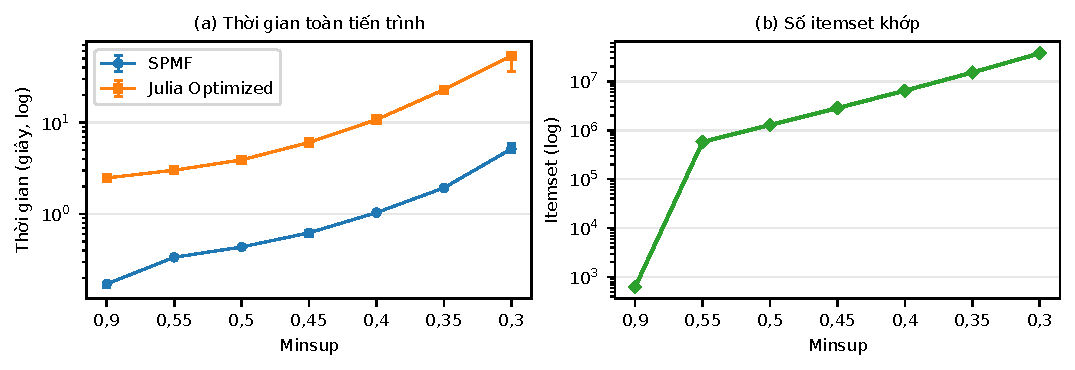
\includegraphics[width=\textwidth]{benchmark-chess.pdf}
\caption{Chess theo minsup. (a) Median thời gian toàn tiến trình cold, thanh sai
số min--max từ ba lần chạy. (b) Số itemset khớp.}
\label{fig:c2-1}
\end{figure*}

\begin{figure*}[!t]
\centering
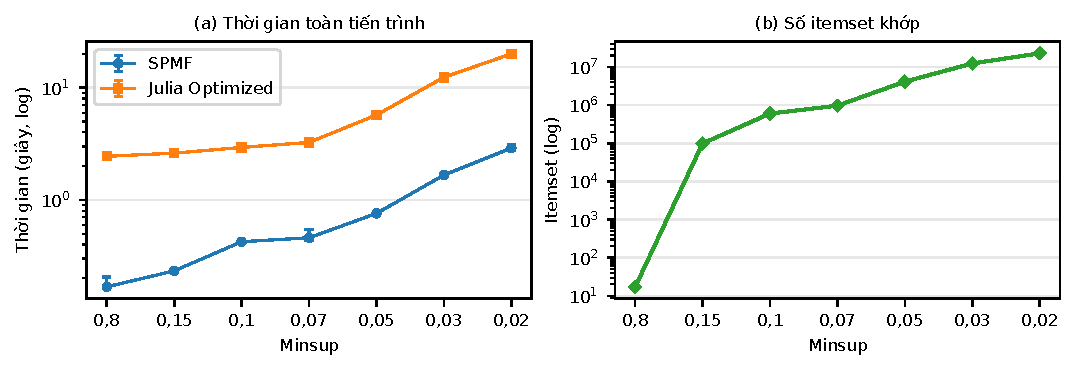
\includegraphics[width=\textwidth]{benchmark-mushroom.pdf}
\caption{Mushroom theo minsup. (a) Median thời gian toàn tiến trình cold, thanh
sai số min--max từ ba lần chạy. (b) Số itemset khớp.}
\label{fig:c2-2}
\end{figure*}

\begin{figure*}[!t]
\centering
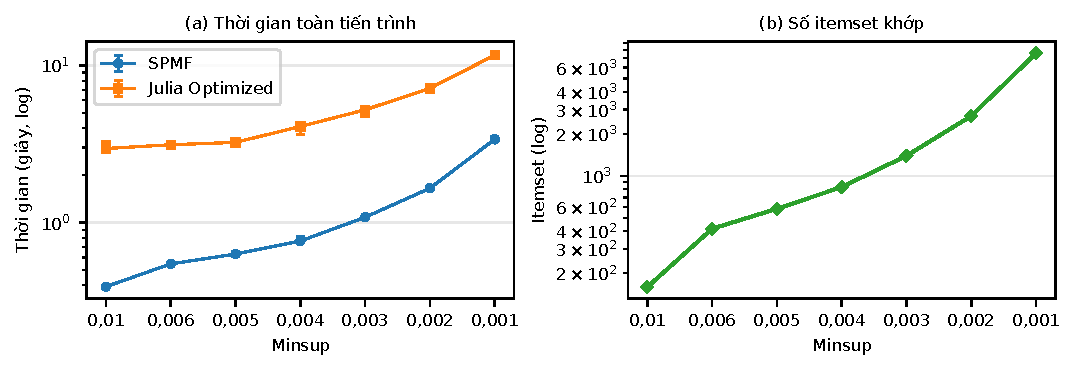
\includegraphics[width=\textwidth]{benchmark-retail.pdf}
\caption{Retail theo minsup. (a) Median thời gian toàn tiến trình cold, thanh sai
số min--max từ ba lần chạy. (b) Số itemset khớp.}
\label{fig:c2-3}
\end{figure*}

\begin{figure*}[!t]
\centering
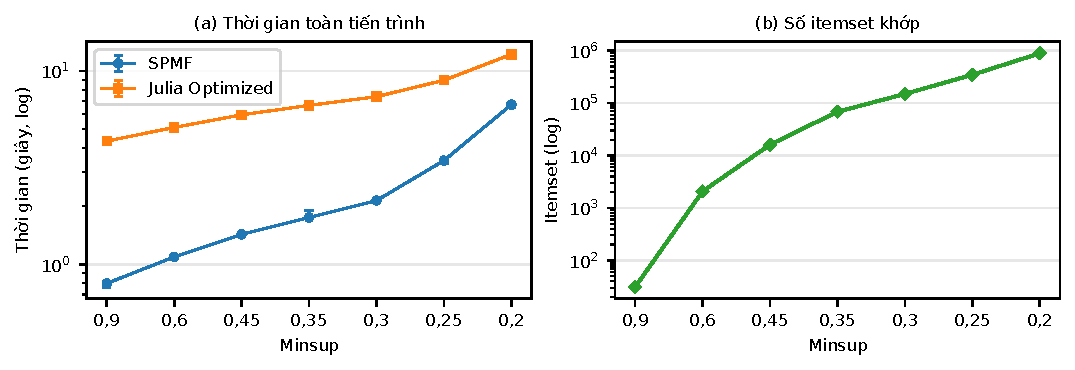
\includegraphics[width=\textwidth]{benchmark-accidents.pdf}
\caption{Accidents theo minsup. (a) Median thời gian toàn tiến trình cold, thanh
sai số min--max từ ba lần chạy. (b) Số itemset khớp.}
\label{fig:c2-4}
\end{figure*}

\begin{figure*}[!t]
\centering
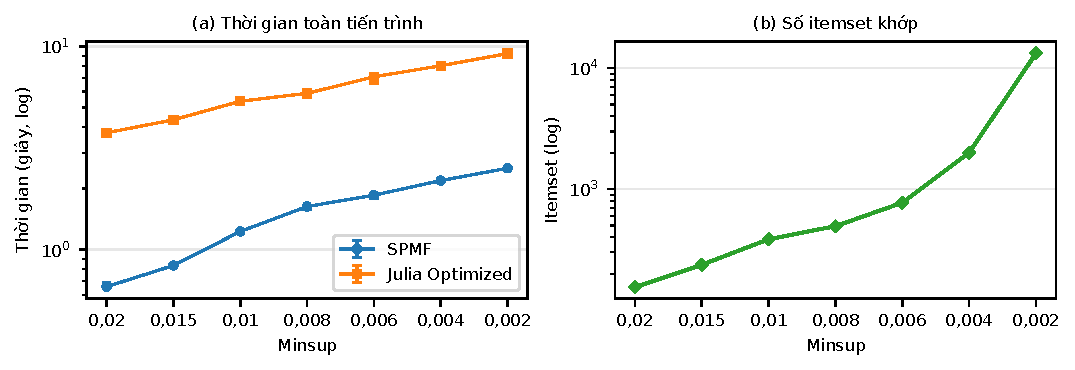
\includegraphics[width=\textwidth]{benchmark-t10i4d100k.pdf}
\caption{T10I4D100K theo minsup. (a) Median thời gian toàn tiến trình cold, thanh
sai số min--max từ ba lần chạy. (b) Số itemset khớp.}
\label{fig:c2-5}
\end{figure*}

Hình~\ref{fig:c2-6} trực quan hóa Bảng~\ref{tab:c2-VI}. Chênh lệch peak working set giữa SPMF và Julia Optimized ở mức minsup thứ tư lớn hơn trên Accidents và T10I4D100K so với Chess và Mushroom, dù hai tập sau có thể sinh nhiều mẫu hơn. Số mẫu đầu ra vì vậy chỉ là một trong các biến cần xem xét khi diễn giải mức dùng bộ nhớ.

\begin{figure*}[!t]
\centering
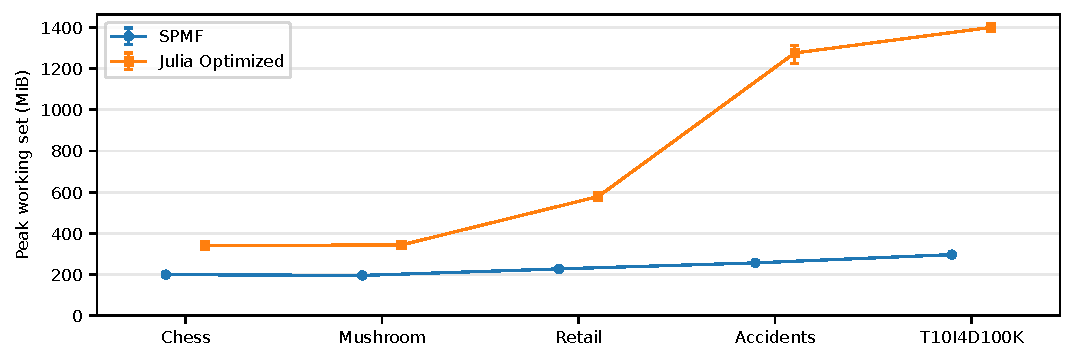
\includegraphics[width=\textwidth]{benchmark-rss.pdf}
\caption{Median peak working set trên Windows ở mức minsup thứ tư. Thanh sai số
biểu thị min--max của ba process mới. Chỉ số bao gồm bộ nhớ của runtime.}
\label{fig:c2-6}
\end{figure*}

Ở ngưỡng thấp nhất, Chess sinh 37,28 triệu itemset và Mushroom sinh 22,84 triệu. Việc định dạng và ghi số lượng mẫu này có thể đóng góp đáng kể vào wall time. Thực nghiệm gộp các giai đoạn trong cùng phép đo nên chưa tách được thời gian khai thác. Trên Retail và T10I4D100K, peak working set của Julia tăng khi hạ minsup. Cần đo heap theo pha để xác định phần tăng có liên quan đến bitmap hoặc cấu trúc nào khác.

Hình~\ref{fig:c2-7} minh họa phần scalability Baseline--Optimized ở Bảng~\ref{tab:c2-IV}. Với T10I4D100K, Optimized nhanh hơn ở cả năm phần tiền tố, còn peak RSS cao hơn ở 75\% và 100\%. Đợt đo SPMF--Julia dùng dữ liệu toàn tập. Các đường scalability đều là số liệu ngày 19-11.

\begin{figure*}[!t]
\centering
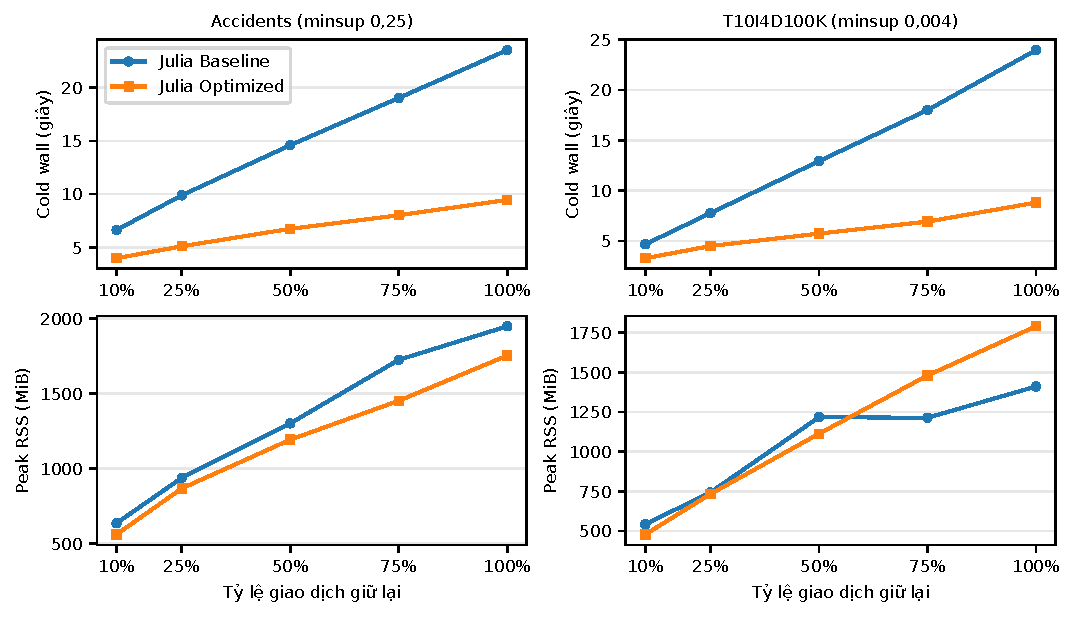
\includegraphics[width=\textwidth]{benchmark-scalability.pdf}
\caption{Scalability Baseline--Optimized trên Accidents và T10I4D100K. Mỗi điểm
là median ba lần cold trên cùng phần tiền tố dữ liệu.}
\label{fig:c2-7}
\end{figure*}

Ba lần lặp trên một máy chỉ cho phép mô tả kết quả tại cấu hình đã đo. Chẳng hạn tại Chess, minsup 0,3, thời gian Julia dao động 36,420--57,130 giây và cả ba lần đều được giữ. Đợt đo tiếp tục từ checkpoint sau giới hạn hai giờ của harness, với cùng fingerprint và các phép đo cũ được giữ nguyên. Dữ liệu dùng snapshot tải từ SPMF theo manifest. Các bản sao Hugging Face hoặc Kaggle khớp checksum vẫn chưa được xác minh. Gói bàn giao lưu digest và bằng chứng kiểm tra output.

\subsection{Ảnh hưởng của độ dài giao dịch}

Pilot dữ liệu tổng hợp giữ cố định 10.000 giao dịch, 512 ID có thể xuất hiện, seed 20261125 và minsup 0,008. Mỗi giao dịch được cắt thành các tiền tố dài 5, 10, 20 hoặc 40 của cùng một hoán vị ngẫu nhiên. Chạy Windows 11 trên Intel Core i7-11800H với Julia 1.12.0 một luồng. Đo warm count gồm chuẩn hóa, dựng cây, thu Nodeset và khai thác qua callback. Sau warm-up, mỗi biến thể chạy ba lần ở mỗi độ dài. Hai kết quả khớp từng itemset và support ở cả bốn độ dài.

\begin{table*}[!t]
\centering\footnotesize
\caption{Pilot độ dài giao dịch. Thời gian là median {[}min--max{]} của ba lượt
warm count, đơn vị giây.}
\label{tab:c2-VII}
\setlength{\tabcolsep}{4pt}
\begin{tabular}{rrrrrr}
\hline
\textbf{Item/giao dịch} & \textbf{Node BMC} & \textbf{Bản ghi quét} & \textbf{Itemset} & \textbf{Baseline (s)} & \textbf{Optimized (s)} \\ \hline
5 & 37.638 & 10.592.198 & 496 & 1,557 {[}1,481--1,631{]} & 0,343 {[}0,318--0,359{]} \\
10 & 86.572 & 24.000.798 & 512 & 3,843 {[}3,554--3,898{]} & 0,892 {[}0,795--0,977{]} \\
20 & 183.235 & 49.244.166 & 512 & 7,457 {[}7,214--7,621{]} & 1,646 {[}1,612--1,650{]} \\
40 & 378.929 & 100.444.039 & 1.365 & 17,211 {[}17,124--18,498{]} & 3,644 {[}3,553--3,681{]} \\
\hline
\end{tabular}
\end{table*}

Bảng~\ref{tab:c2-VII} cho thấy khi tăng từ 10 lên 20 item/giao dịch, đầu ra giữ nguyên 512 mẫu, trong khi số node BMC tăng 2,12 lần, số bản ghi quét tăng 2,05 lần và thời gian tăng ở cả hai biến thể. Ở mức 40 item, số mẫu cũng tăng, nên mức tăng thời gian đi cùng cả sự thay đổi về cấu trúc đầu vào và lượng kết quả sinh ra. Pilot dùng một seed, một máy và chỉ mô tả phạm vi warm count.

% Sinh tự động từ docs/report/chapter3.md bởi build.py — sửa file Markdown, không sửa file này.
\section{Ứng dụng}\label{sec:ch3}

Chương này áp dụng cài đặt negFIN của nhóm \cite{negfin} cho hai bài toán thực tế theo yêu cầu đề: phân tích giỏ hàng trên dữ liệu bán lẻ và tìm pattern trên chuỗi DNA. Mọi frequent itemset đều do CLI \texttt{run.jl} của nhóm sinh ra (Baseline); Python chỉ dùng để chuyển dữ liệu gốc sang định dạng SPMF và hậu xử lý kết quả. Toàn bộ pipeline chạy lại được bằng notebook \nolinkurl{notebooks/demo.ipynb}.

\subsection{Quy trình chung}

Mỗi ứng dụng gồm bốn bước: (1) tải dữ liệu công khai và kiểm SHA-256 theo \nolinkurl{data/applications/manifest.toml}; (2) script \texttt{prepare.py} biến dữ liệu gốc thành file transaction SPMF (mỗi dòng một giao dịch, item là số nguyên dương) cùng bảng ánh xạ ID $\leftrightarrow$ ý nghĩa; (3) chạy negFIN với \texttt{minsup} là tỷ lệ thập phân, ngưỡng tuyệt đối \(m = \lceil \mathit{minsup}\cdot N\rceil\) với \(N\) là số transaction; (4) hậu xử lý: sinh luật kết hợp (ứng dụng A) hoặc so sánh pattern giữa các lớp (ứng dụng B), rồi giải mã ID thành tên để diễn giải.

Cả hai bộ dữ liệu lấy từ UCI Machine Learning Repository, giấy phép CC BY 4.0; dữ liệu gốc không đưa vào repo mà được notebook tải và kiểm checksum khi chạy.

\subsection{Ứng dụng 1 --- Phân tích giỏ hàng (Online Retail)}

\subsubsection{Mục tiêu}

Tìm các nhóm sản phẩm thường được mua cùng nhau và sinh luật kết hợp X $\Rightarrow$ Y để gợi ý bán kèm, đóng gói combo và bố trí trưng bày.

\subsubsection{Dữ liệu}

Online Retail \cite{retail} gồm 541.909 dòng hóa đơn của một cửa hàng trực tuyến tại Anh chuyên quà tặng, từ 01/12/2010 đến 09/12/2011 (DOI 10.24432/C5BW33). Mỗi dòng có \texttt{InvoiceNo}, \texttt{StockCode}, \texttt{Description}, \texttt{Quantity}, \texttt{InvoiceDate}, \texttt{UnitPrice}, \texttt{CustomerID}, \texttt{Country}. Theo mô tả của UCI, nhiều khách hàng của công ty là người bán sỉ.

\subsubsection{Tạo transaction}

Một hóa đơn là một transaction; item là \texttt{StockCode} sản phẩm (chuẩn hóa chữ hoa, trùng trong hóa đơn tính một lần). Bảng~\ref{tab:c3-I} liệt kê các bước lọc theo thứ tự.

\begin{table*}[!t]
\centering\footnotesize
\caption{Các bước lọc dữ liệu Online Retail}
\label{tab:c3-I}
\setlength{\tabcolsep}{4pt}
\begin{tabular}{llrr}
\hline
\textbf{Bước lọc} & \textbf{Lý do} & \textbf{Dòng} & \textbf{Hóa đơn} \\ \hline
Dữ liệu gốc &  & 541.909 & 25.900 \\
Bỏ hóa đơn không toàn số (\texttt{C…} hủy, \texttt{A…} điều chỉnh) & không phải giao dịch mua & 532.618 & 22.061 \\
Bỏ \texttt{Quantity} $\le$ 0 & trả hàng, ghi nhận hỏng & 531.282 & 20.725 \\
Bỏ \texttt{UnitPrice} $\le$ 0 & điều chỉnh kho & 530.103 & 19.959 \\
Chỉ giữ mã dạng \texttt{\textbackslash{}d\{5\}{[}A-Z{]}*} & bỏ phí vận chuyển, phí ngân hàng, voucher\ldots{} & 527.725 & 19.773 \\
\hline
\end{tabular}
\end{table*}

Kết quả có N = 19.773 transaction, 3.791 sản phẩm khác nhau, trung bình 26,2 sản phẩm mỗi hóa đơn. Các dòng thiếu \texttt{CustomerID} được giữ lại vì phân tích giỏ hàng chỉ cần nội dung hóa đơn. Sản phẩm được đánh ID theo thứ tự sắp xếp của mã, nên ánh xạ ổn định với cùng dữ liệu và quy tắc lọc; tên hiển thị là mô tả xuất hiện nhiều nhất của mỗi mã.

\subsubsection{Sinh luật kết hợp}

Với mỗi frequent itemset \(Z\) có ít nhất hai phần tử, sinh mọi luật \(X \Rightarrow Y\) với \(X \cup Y = Z\), \(X\) và \(Y\) khác rỗng và rời nhau. Gọi \(\sup(\cdot)\) là số transaction chứa tập đó và \(N\) là tổng số transaction; các độ đo là \cite{agrawal}, \cite{brin}:

\begin{equation}
\mathrm{supp}(X \Rightarrow Y) = \frac{\sup(X \cup Y)}{N},
\end{equation}

\begin{equation}
\mathrm{conf}(X \Rightarrow Y) = \frac{\sup(X \cup Y)}{\sup(X)},
\end{equation}

\begin{equation}
\mathrm{lift}(X \Rightarrow Y) = \frac{\mathrm{conf}(X \Rightarrow Y)}{\sup(Y)/N}.
\end{equation}

Lift lớn hơn 1 nghĩa là \(X\) và \(Y\) cùng xuất hiện nhiều hơn so với khi chúng độc lập.

Do mọi tập con của một frequent itemset cũng frequent, \(\sup(X)\) và \(\sup(Y)\) đều có sẵn trong output của negFIN, không cần quét lại dữ liệu. Phép tính được kiểm bằng ví dụ tính tay trên CSDL toy 5 giao dịch của nhóm: luật \(\{2\} \Rightarrow \{3\}\) có \(\sup(\{2,3\}) = 3\), \(\sup(\{2\}) = \sup(\{3\}) = 4\), nên confidence \(= 0{,}75\) và lift \(= 0{,}75/0{,}8 = 0{,}9375\); với minconf \(= 0\), 15 frequent itemset sinh đúng 50 luật (mỗi itemset \(k\) phần tử cho \(2^k - 2\) luật).

\subsubsection{Tham số và kết quả}

Bảng~\ref{tab:c3-II} cho thấy số mẫu tăng nhanh khi hạ minsup. Nhóm chọn \textbf{minsup = 0,01} (\(m = 198\) hóa đơn) để có itemset từ ba sản phẩm trở lên, và \textbf{minconf = 0,5}.

\begin{table}[!t]
\centering\footnotesize
\caption{negFIN trên Online Retail (N = 19.773)}
\label{tab:c3-II}
\setlength{\tabcolsep}{3pt}
\begin{tabular}{rrrr}
\hline
\textbf{minsup} & \textbf{min\_count} & \textbf{Số itemset} & \textbf{Dài nhất} \\ \hline
0,03 & 594 & 143 & 2 \\
0,02 & 396 & 395 & 3 \\
0,01 & 198 & 2.026 & 5 \\
\hline
\end{tabular}
\end{table}

Ở minsup 0,01 và minconf 0,5 có 962 luật, sinh từ 477 itemset; lift thấp nhất là 4,74, trung vị 12,03. Bảng~\ref{tab:c3-III} liệt kê mười luật có lift cao nhất. Tất cả thuộc họ sản phẩm HERB MARKER (que cắm đánh dấu chậu thảo mộc) và là các cách chia X/Y khác nhau của chỉ ba itemset: \{THYME, ROSEMARY, PARSLEY\} (luật 1--4), \{THYME, ROSEMARY, BASIL\} (5--8) và \{THYME, ROSEMARY\} (9--10); hai luật cùng một itemset có cùng support nhưng khác confidence vì mẫu số sup(X) khác nhau.

\begin{table}[!t]
\centering\footnotesize
\caption{Mười luật có lift cao nhất (minsup 0,01, minconf 0,5). Mọi sản phẩm là
HERB MARKER; chỉ ghi tên loại cây}
\label{tab:c3-III}
\setlength{\tabcolsep}{3pt}
\begin{tabular}{rlrrr}
\hline
\textbf{\#} & \textbf{X $\Rightarrow$ Y} & \textbf{Supp.} & \textbf{Conf.} & \textbf{Lift} \\ \hline
1 & THYME $\Rightarrow$ ROSEMARY + PARSLEY & 1,03\% (203) & 0,86 & 78,77 \\
2 & ROSEMARY + PARSLEY $\Rightarrow$ THYME & 1,03\% (203) & 0,94 & 78,77 \\
3 & THYME + PARSLEY $\Rightarrow$ ROSEMARY & 1,03\% (203) & 0,95 & 78,52 \\
4 & ROSEMARY $\Rightarrow$ THYME + PARSLEY & 1,03\% (203) & 0,85 & 78,52 \\
5 & THYME + BASIL $\Rightarrow$ ROSEMARY & 1,01\% (200) & 0,95 & 78,46 \\
6 & ROSEMARY $\Rightarrow$ THYME + BASIL & 1,01\% (200) & 0,83 & 78,46 \\
7 & ROSEMARY + BASIL $\Rightarrow$ THYME & 1,01\% (200) & 0,93 & 77,97 \\
8 & THYME $\Rightarrow$ ROSEMARY + BASIL & 1,01\% (200) & 0,84 & 77,97 \\
9 & THYME $\Rightarrow$ ROSEMARY & 1,12\% (221) & 0,93 & 76,83 \\
10 & ROSEMARY $\Rightarrow$ THYME & 1,12\% (221) & 0,92 & 76,83 \\
\hline
\end{tabular}
\end{table}

Vì Bảng~\ref{tab:c3-III} chỉ cho thấy một họ sản phẩm, Bảng~\ref{tab:c3-IV} dùng thêm một quy tắc khách quan để minh họa nhiều nhóm hơn: duyệt danh sách luật theo lift giảm dần, chỉ giữ luật không chứa sản phẩm nào đã xuất hiện ở các luật được giữ trước đó.

\begin{table*}[!t]
\centering\footnotesize
\caption{Mười luật lift cao nhất không trùng sản phẩm (minsup 0,01, minconf 0,5)}
\label{tab:c3-IV}
\setlength{\tabcolsep}{4pt}
\begin{tabular}{rlrrr}
\hline
\textbf{\#} & \textbf{X $\Rightarrow$ Y} & \textbf{Supp.} & \textbf{Conf.} & \textbf{Lift} \\ \hline
1 & HERB MARKER THYME $\Rightarrow$ HERB MARKER ROSEMARY + PARSLEY & 1,03\% & 0,86 & 78,77 \\
2 & HERB MARKER MINT $\Rightarrow$ HERB MARKER BASIL & 1,05\% & 0,87 & 70,81 \\
3 & REGENCY TEA PLATE PINK $\Rightarrow$ REGENCY TEA PLATE ROSES + GREEN & 1,29\% & 0,84 & 51,82 \\
4 & SET OF 3 WOODEN TREE DECORATIONS $\Rightarrow$ SET OF 3 WOODEN STOCKING
DECORATION & 1,11\% & 0,75 & 46,33 \\
5 & REGENCY SUGAR BOWL GREEN $\Rightarrow$ REGENCY MILK JUG PINK & 1,23\% & 0,75 & 45,36 \\
6 & POPPY'S PLAYHOUSE LIVINGROOM $\Rightarrow$ POPPY'S PLAYHOUSE BEDROOM +
KITCHEN & 1,13\% & 0,68 & 43,14 \\
7 & JAM JAR WITH GREEN LID $\Rightarrow$ JAM JAR WITH PINK LID & 1,15\% & 0,74 & 42,94 \\
8 & PINK POLKADOT CUP $\Rightarrow$ BLUE POLKADOT CUP & 1,05\% & 0,68 & 41,22 \\
9 & CHILDRENS CUTLERY DOLLY GIRL $\Rightarrow$ CHILDRENS CUTLERY SPACEBOY & 1,15\% & 0,76 & 40,97 \\
10 & BLUE POLKADOT BOWL $\Rightarrow$ PINK POLKADOT BOWL & 1,05\% & 0,65 & 38,36 \\
\hline
\end{tabular}
\end{table*}

Hình~\ref{fig:c3-1} cho thấy phân bố của toàn bộ 962 luật: 93,7\% có support dưới 2\% và 79,1\% có lift dưới 20. Ba mươi hai luật có lift từ 60 trở lên đều thuộc họ HERB MARKER và có support không quá 1,12\%, nằm ở góc trái trên của hình; luật có support cao nhất (4,17\%, chứa JUMBO BAG PINK POLKADOT) chỉ có lift trung bình. Như vậy luật có lift cao nhất không phải luật phổ biến nhất.

\begin{figure}[!t]
\centering
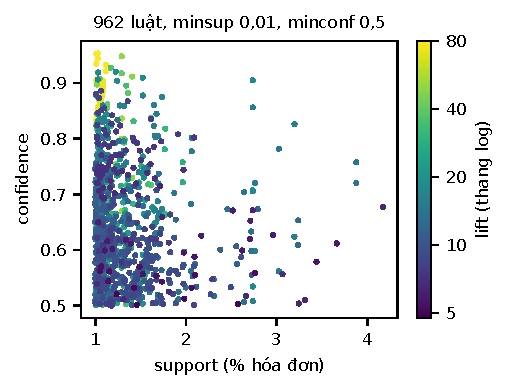
\includegraphics[width=\columnwidth]{retail-rules.pdf}
\caption{Support và confidence của 962 luật (minsup 0,01, minconf 0,5); màu biểu
diễn lift theo thang log.}
\label{fig:c3-1}
\end{figure}

\subsubsection{Diễn giải}

Các luật thể hiện hai kiểu hành vi mua:

\begin{itemize}
\tightlist
\item
  \textbf{Mua trọn bộ sưu tập} (herb marker, Poppy's Playhouse, đồ trang trí gỗ Giáng sinh): khách mua một mẫu thường mua tiếp các mẫu cùng dòng. Cửa hàng có thể bán theo bộ, hiển thị ``các mẫu còn lại trong bộ'' trên trang sản phẩm và trưng bày cạnh nhau.
\item
  \textbf{Phối nhiều màu của cùng một thiết kế} (bộ Regency, hũ mứt, cốc và bát polkadot, dao dĩa trẻ em bản girl/boy): khách lấy nhiều biến thể màu cùng lúc. Gợi ý là gói ``mix màu'' và nhập kho các màu theo tỷ lệ đi cùng nhau, tránh hết một màu làm mất cả đơn.
\end{itemize}

Confidence 0,65--0,95 nghĩa là phần lớn hóa đơn có vế trái cũng có vế phải; lift 38--79 cho biết các sản phẩm này xuất hiện cùng nhau nhiều gấp hàng chục lần so với khi được mua độc lập.

\subsubsection{Giới hạn}

Dữ liệu chỉ của một nhà bán lẻ trong một năm, và vì nhiều khách là người bán sỉ nên luật phản ánh hành vi nhập hàng theo bộ nhiều hơn người tiêu dùng lẻ. Lift nhạy với sản phẩm hiếm: support riêng của các sản phẩm trong Bảng~\ref{tab:c3-III} và \ref{tab:c3-IV} chỉ khoảng 1,2--1,9\%, nên cần đọc lift cùng support và confidence. minsup 0,01 bỏ qua sản phẩm có ít hơn 198 hóa đơn, do đó không thấy luật của mặt hàng ngách. Cuối cùng, luật chỉ thể hiện đồng xuất hiện, không phải quan hệ nhân quả.

\subsection{Ứng dụng 2 --- Pattern trên chuỗi DNA (Splice-junction)}

\subsubsection{Mục tiêu}

Kiểm tra xem negFIN có tự tìm ra các tín hiệu trình tự đặc trưng ở vị trí cắt nối (splice junction) hay không, bằng cách khai thác pattern riêng từng lớp chuỗi rồi so sánh giữa các lớp.

\subsubsection{Dữ liệu}

Bộ Splice-junction Gene Sequences \cite{splice} (DOI 10.24432/C5M888) gồm 3.190 chuỗi DNA linh trưởng lấy từ GenBank 64.1, mỗi chuỗi 60 base, ứng với vị trí −30 đến −1 và +1 đến +30; điểm nối nằm giữa −1 và +1. Có ba lớp: EI --- ranh giới exon$\rightarrow$intron (donor), 767 chuỗi; IE --- ranh giới intron$\rightarrow$exon (acceptor), 768 chuỗi; N --- không phải điểm nối, 1.655 chuỗi. File mô tả của nguồn ghi ngược donor/acceptor ở một mục; chương này dùng cách gọi khớp với phần mô tả bài toán của nguồn và với sinh học: EI là donor, IE là acceptor.

\subsubsection{Tạo transaction}

Mỗi chuỗi \(s\) là một transaction \(T(s)\); item là cặp vị trí--base, ký hiệu \texttt{p\textless{}vị\ trí\textgreater{}\_\textless{}base\textgreater{}}. Ví dụ, chuỗi EI đầu tiên của tập dữ liệu (ATRINS-DONOR-521) bắt đầu bằng \texttt{CCA…}, có \texttt{G} ở −1, \texttt{GT} ở +1..+2 và kết thúc bằng \texttt{G}, nên \(T(s)\) = \{\texttt{p-30\_C}, \texttt{p-29\_C}, \texttt{p-28\_A}, \ldots, \texttt{p-1\_G}, \texttt{p+1\_G}, \texttt{p+2\_T}, \ldots, \texttt{p+30\_G}\}, gồm 60 item. Với 60 vị trí và 4 base có 240 item; ID cố định \(\mathit{id} = 4j + b + 1\), với \(j \in \{0,\ldots,59\}\) là chỉ số vị trí và \(b \in \{0,1,2,3\}\) là chỉ số base theo thứ tự A, C, G, T, nên ánh xạ không phụ thuộc dữ liệu. Base mơ hồ (N, D, S, R; xuất hiện ở 15 chuỗi) không sinh item tại vị trí đó, nên các chuỗi này có ít hơn 60 item. Mã hóa kèm vị trí khiến mỗi transaction có tối đa một item cho mỗi vị trí, giữ được thông tin ``base nào ở vị trí nào'' dù itemset là tập hợp không có thứ tự. Các chuỗi trùng của nguồn (185 chuỗi) được giữ nguyên và được đếm như các transaction riêng.

Gọi \(D_c\) là tập chuỗi của lớp \(c \in \{\mathrm{EI}, \mathrm{IE}, \mathrm{N}\}\). negFIN chạy riêng trên từng \(D_c\) với ngưỡng \(m_c = \lceil \mathit{minsup}\cdot|D_c|\rceil\), và support theo lớp của itemset \(I\) được tính trên đúng mẫu số của lớp đó:

\begin{equation}
\mathrm{supp}_c(I) = \frac{|\{s \in D_c : I \subseteq T(s)\}|}{|D_c|}.
\end{equation}

Để so sánh, với mỗi itemset \(I\) của lớp đích \(c\), nhóm đếm lại \(\mathrm{supp}_{c'}(I)\) ở cả ba lớp trực tiếp từ transaction và tính độ tăng (growth) \cite{dongli} so với các lớp còn lại gộp chung \(D_{\neg c} = \bigcup_{c' \neq c} D_{c'}\):

\begin{equation}
\mathrm{growth}_c(I) = \frac{\mathrm{supp}_c(I)}{\mathrm{supp}_{\neg c}(I)},
\end{equation}

trong đó \(\mathrm{supp}_{\neg c}(I)\) tính theo công thức trên với mẫu số \(|D_{\neg c}|\); growth \(= \infty\) khi \(I\) không xuất hiện ở lớp nào khác. Vì lớp N có số chuỗi gấp khoảng hai lần EI hoặc IE, \(\mathrm{supp}_{\neg c}\) là tỷ lệ có trọng số theo kích thước lớp, không phải trung bình cộng của hai tỷ lệ.

\subsubsection{Tham số và kết quả}

\begin{table}[!t]
\centering\footnotesize
\caption{Số itemset theo lớp và minsup}
\label{tab:c3-V}
\setlength{\tabcolsep}{3pt}
\begin{tabular}{lrrrr}
\hline
\textbf{Lớp} & \textbf{N chuỗi} & \textbf{minsup 0,5} & \textbf{0,3} & \textbf{0,2} \\ \hline
EI & 767 & 35 & 280 & 2.375 \\
IE & 768 & 7 & 331 & 1.284 \\
N & 1.655 & 0 & 0 & 240 \\
\hline
\end{tabular}
\end{table}

Bảng~\ref{tab:c3-V} cho số itemset của từng lớp ở ba mức minsup. Nhóm chọn \textbf{minsup = 0,3} cho phân tích chính. Lớp N không có itemset nào ở 0,3; ở 0,2 có đủ 240 item đơn (mỗi base ở mỗi vị trí chiếm khoảng 25\%) nhưng không có cặp nào. Lớp N vì vậy đóng vai trò đối chứng: chuỗi không phải điểm nối không có tín hiệu gắn với vị trí.

Ở minsup 0,5, các item có mặt ở ít nhất một nửa số chuỗi là: với EI, \texttt{p-2\_A} (58\%), \texttt{p-1\_G} (81\%), \texttt{p+1\_G} (99,7\%), \texttt{p+2\_T} (99,0\%), \texttt{p+4\_A} (72\%), \texttt{p+5\_G} (86\%); với IE, \texttt{p-3\_C} (79\%), \texttt{p-2\_A} (99,6\%), \texttt{p-1\_G} (99,7\%).

Hình~\ref{fig:c3-2} tóm tắt tần suất của từng base ở từng vị trí trong mỗi lớp. Mỗi ô là support của một itemset một phần tử \texttt{p\textless{}vị\ trí\textgreater{}\_\textless{}base\textgreater{}} trong lớp đó, đếm trực tiếp từ transaction để có đủ 240 item; hình chỉ mang tính mô tả và giúp đọc các itemset nhiều phần tử ở Bảng~\ref{tab:c3-VI}. Ở EI, các ô đậm tập trung ở −1 (G), +1 (G), +2 (T) và +5 (G); ở IE, ở −3 (C), −2 (A), −1 (G), cùng một dải C/T nhạt hơn trải từ khoảng −20 đến −5; lớp N gần như đồng đều.

\begin{figure*}[!t]
\centering
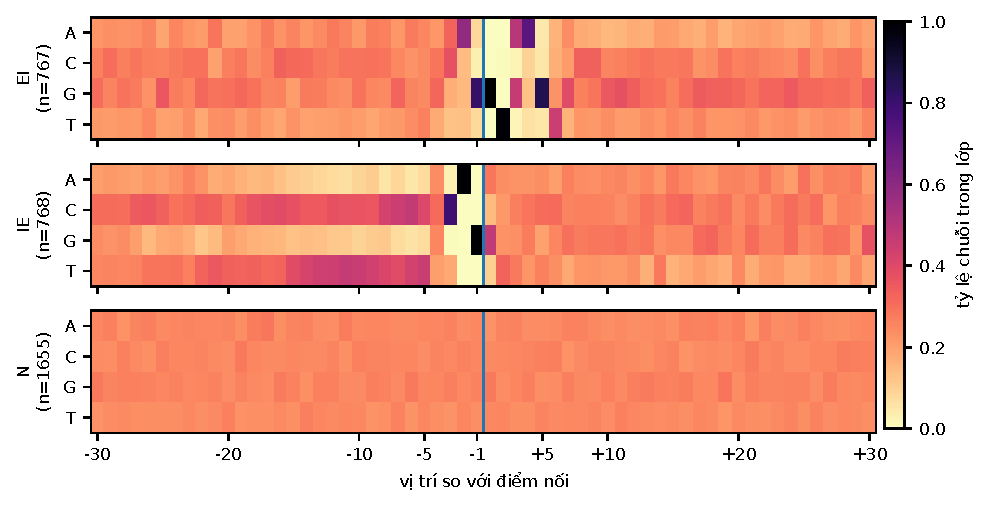
\includegraphics[width=\textwidth]{splice-positions.pdf}
\caption{Tỷ lệ chuỗi có mỗi base tại mỗi vị trí, theo lớp. Đường dọc đánh dấu
điểm nối giữa −1 và +1.}
\label{fig:c3-2}
\end{figure*}

Bảng~\ref{tab:c3-VI} liệt kê các itemset có growth cao nhất của EI và IE.

\begin{table*}[!t]
\centering\footnotesize
\caption{Itemset có growth cao nhất của mỗi lớp (minsup 0,3); support tính theo
từng lớp}
\label{tab:c3-VI}
\setlength{\tabcolsep}{4pt}
\begin{tabular}{llrrrr}
\hline
\textbf{Lớp} & \textbf{Itemset} & \textbf{EI} & \textbf{IE} & \textbf{N} & \textbf{Growth} \\ \hline
EI & p+1\_G p+2\_T p+4\_A p+5\_G p+6\_T & 30,2\% & 0,0\% & 0,0\% & $\infty$ \\
EI & p+1\_G p+2\_T p+5\_G p+6\_T & 40,3\% & 0,1\% & 0,1\% & 488 \\
EI & p+1\_G p+2\_T p+4\_A p+5\_G & 63,8\% & 0,9\% & 0,1\% & 193 \\
EI & p-1\_G p+1\_G p+2\_T p+4\_A p+5\_G & 47,3\% & 0,9\% & 0,0\% & 164 \\
IE & p-12\_T p-3\_C p-2\_A p-1\_G & 3,4\% & 33,2\% & 0,4\% & 25,1 \\
IE & p-10\_T p-3\_C p-2\_A p-1\_G & 2,9\% & 32,9\% & 0,6\% & 24,9 \\
IE & p-11\_T p-3\_C p-2\_A p-1\_G & 3,8\% & 37,1\% & 0,7\% & 22,5 \\
IE & p-7\_C p-3\_C p-2\_A p-1\_G & 5,1\% & 35,9\% & 0,3\% & 19,8 \\
\hline
\end{tabular}
\end{table*}

\subsubsection{Diễn giải}

Kết quả được đối chiếu với trình tự consensus đã công bố cho intron loại GT-AG: donor \texttt{MAG\textbar{}GTRAGT} và acceptor \texttt{(Y)n\ N\ CAG\textbar{}G} \cite{shapiro}.

\begin{itemize}
\tightlist
\item
  \textbf{Donor (EI).} negFIN tìm lại gần như đủ consensus donor: \texttt{G} ở −1 (kèm \texttt{A} ở −2) phía exon, \texttt{GT} ở +1..+2, rồi \nolinkurl{A/G} ở +3, \texttt{A} ở +4, \texttt{G} ở +5, \texttt{T} ở +6. Riêng cặp \texttt{GT} ở +1..+2 có mặt ở 99,0\% chuỗi EI, so với 14,1\% ở IE và 5,9\% ở N. Itemset năm phần tử \texttt{p+1\_G\ p+2\_T\ p+4\_A\ p+5\_G\ p+6\_T} xuất hiện ở 30,2\% chuỗi EI và không có ở lớp nào khác.
\item
  \textbf{Acceptor (IE).} Bộ ba \texttt{CAG} ở −3..−1 có mặt ở 78,8\% chuỗi IE, so với 22,8\% ở EI và 2,3\% ở N; riêng \texttt{AG} ở −2..−1 đạt 99,5\%. Các itemset đặc trưng nhất của IE ghép \texttt{CAG} với một base \texttt{T} hoặc \texttt{C} ở vị trí −6..−17, tức vùng giàu pyrimidine (polypyrimidine tract) nằm trước acceptor. Kiểm tra trực tiếp: tỷ lệ pyrimidine ở vùng −20..−5 là 77,4\% với IE, so với 49,1\% với EI và 49,3\% với N.
\item
  Growth của IE thấp hơn EI vì tín hiệu acceptor phân tán: vùng pyrimidine không cố định vị trí nên mỗi vị trí chỉ đạt khoảng 30--40\%, trong khi tín hiệu donor tập trung ở vài vị trí gần như cố định.
\end{itemize}

\subsubsection{Giới hạn}

Itemset chỉ biểu diễn đồng xuất hiện của các base ở vị trí tuyệt đối, không có thứ tự hay khoảng cách tương đối; vì vậy một motif có thể dịch vị trí như polypyrimidine tract bị tách thành nhiều itemset rời rạc. Growth chỉ mô tả mức đặc trưng trên chính dữ liệu này: không có tập kiểm tra riêng, không có kiểm định thống kê, nên không phải bằng chứng về khả năng phân lớp chuỗi mới; growth = $\infty$ của itemset EI trong Bảng~\ref{tab:c3-VI} cũng chỉ có nghĩa là không quan sát thấy ở 2.423 chuỗi IE và N (768 + 1.655). Các chuỗi trùng được đếm nhiều lần nên support có thể lệch nhẹ so với tập chuỗi duy nhất. Dữ liệu từ năm 1991, chỉ gồm gen linh trưởng và điểm nối GT-AG, nên không suy rộng cho loài khác hay các loại intron hiếm. Chương này chỉ khẳng định các pattern khớp với consensus đã công bố; các pattern còn lại được xem là quan sát.

\subsection{Tái lập và kiểm chứng}

Notebook \nolinkurl{notebooks/demo.ipynb} dùng Julia có sẵn hoặc tự cài Julia 1.12.0 (kiểm SHA-256), lấy mã nguồn ở commit chỉ định, tải hai bộ dữ liệu và kiểm checksum, rồi chạy lần lượt ví dụ toy, ứng dụng 1 và ứng dụng 2 qua \texttt{run.jl}; cell cuối in commit, phiên bản Julia và mọi tham số. Notebook đã được chạy Run all trên runtime Colab mới ở commit \texttt{7e3e9b0} với Julia 1.12.6, cho đúng các số liệu trong chương này; bản có output được chia sẻ công khai tại liên kết trong README. Các bước kiểm chứng đã thực hiện:

\begin{itemize}
\tightlist
\item
  12 unit test Python cho tiền xử lý, sinh luật và so sánh lớp, gồm ví dụ tính tay trên CSDL toy.
\item
  19 luật khác nhau trong Bảng~\ref{tab:c3-III} và \ref{tab:c3-IV} được tính lại support, confidence, lift trực tiếp từ file transaction, không qua negFIN: khớp hoàn toàn.
\item
  Script so sánh lớp đếm lại support của toàn bộ 611 itemset (EI 280, IE 331) từ transaction và báo lỗi nếu khác output của negFIN: không có sai lệch.
\end{itemize}


\section{Kết luận}\label{sec:conclusion}
Trong thực nghiệm so với Baseline, Optimized giảm thời gian cold ở phần lớn cấu hình, với mức dùng bộ nhớ đỉnh tùy dữ liệu và ngưỡng. Trong đợt đo riêng với SPMF, Julia Optimized khớp itemset và support ở cả 35 cấu hình. SPMF có median thời gian và peak working set thấp hơn trong toàn bộ phép đo này. Thời gian bao gồm khởi động, JIT, đọc và ghi nên kết quả mô tả chi phí toàn tiến trình trên máy đo. Pilot độ dài giao dịch cho thấy tăng kích thước mỗi giao dịch có thể làm cây BMC lớn hơn và tăng số bản ghi phải quét ngay cả khi số mẫu đầu ra giữ nguyên. Cùng một cài đặt đã được kiểm chứng qua hai ứng dụng bán lẻ và sinh học.

Hai hướng cải tiến tiếp theo được rút ra từ thực nghiệm: (1) đo heap theo từng giai đoạn và lưu các bitmap ít bit bật bằng cấu trúc thưa để giảm bộ nhớ đỉnh trên dữ liệu thưa; (2) đo riêng chi phí ghi kết quả và ghi theo lô cho các cấu hình sinh hàng chục triệu mẫu như Chess và Mushroom. Với hai ứng dụng, có thể bổ sung kiểm định thống kê cho luật và cho pattern đặc trưng lớp, và mở rộng sang dữ liệu bán lẻ nhiều cửa hàng hoặc bộ gen của các loài khác.

\bibliographystyle{IEEEtran}
\bibliography{refs}

\end{document}
